\newpage
\section{Assignment 2 (50 Points)}
\label{sec:assignment2}

\subsection*{Questions}

\noindent
\textbf{Test your (friend's) ESP}

\noindent
Can you prove or disprove parapsychology using \textit{Signal Detection Theory (SDT)}?

\begin{itemize}
    \item Test at least $n = 2$ (or more if you wish) individuals.
    \item You must provide \textbf{conclusive scientific proof} of ESP capabilities (or lack thereof) for each person tested.
    \item The experimental design may differ across individuals.
    \item Justify all experimental and analysis choices clearly.
\end{itemize}

\vspace{0.5em}
\begin{figure}[h!]
    \centering
    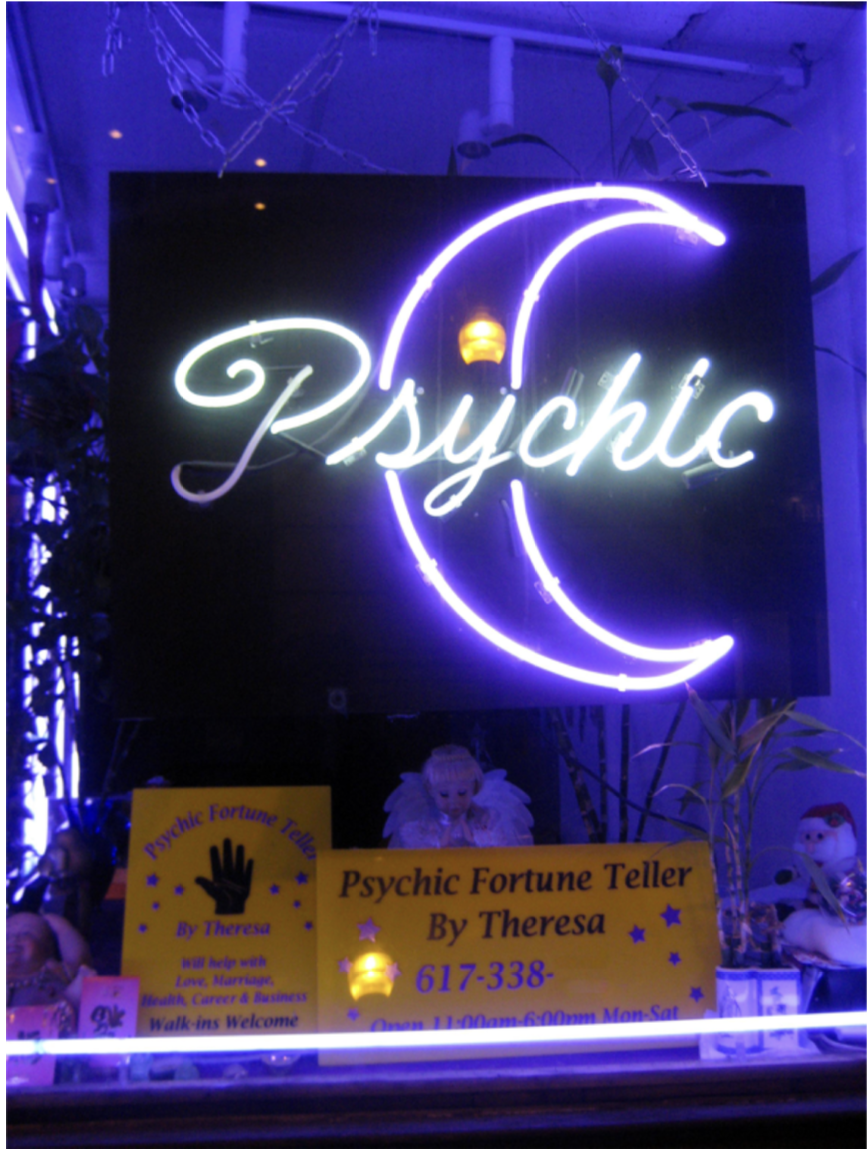
\includegraphics[width=0.8\textwidth]{figures/assignment2.png}
    \caption{Assignment 2 question.}
    \label{fig:assignment2}
\end{figure}

\newpage
\subsection*{Answers}
\noindent\textbf{Experimental Design:} I tested 3 of my friends for ESP capabilities using three different experimental paradigms:

\begin{enumerate}
    \item \textbf{Zener Card Test}: Classic telepathy test using 5 organ symbols (heart, lungs, brain, eye, ear) over 25 trials.
    
    \item \textbf{Binary Choice Test}: Simplified forced-choice paradigm with 2 options (red vs. blue, heads vs. tails, left vs. right, or circle vs. cross) over 50 trials with 50\% chance level. My participant chose circle vs. cross.
    
    \item \textbf{Image Orientation Test}: Clairvoyance test requiring participants to detect whether images were displayed upright or inverted (180° rotation) over 40 trials.
\end{enumerate}

\noindent Each test employed a single-device protocol where a sender viewed the target stimulus and focused on mentally transmitting it to a receiver, who then made their guess without seeing the target. All responses were recorded, and Signal Detection Theory metrics (hits, false alarms, misses, and correct rejections) were calculated.

\begin{itemize}
    \item \textbf{Binary Choice Test (Participant 1):}
    
    \begin{figure}[H]
        \centering
        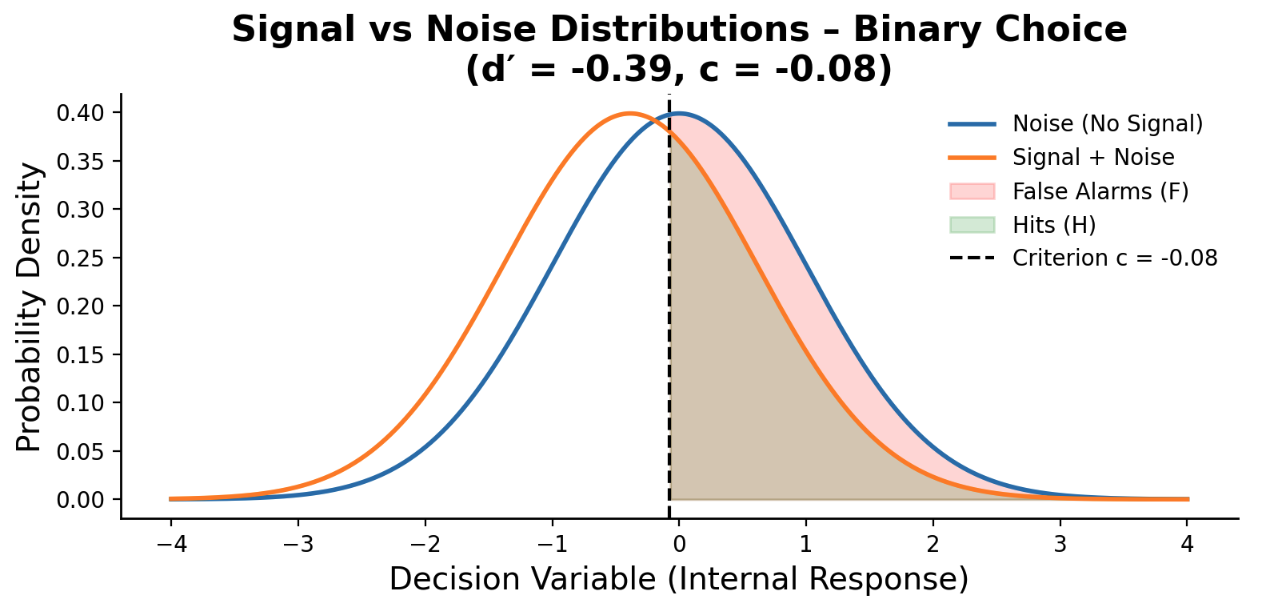
\includegraphics[width=0.75\textwidth]{figures/N_S_AS1.png}
        \caption{Signal and noise distributions in a yes--no detection task.}
        \label{fig:sdt_binary_distributions}
    \end{figure}
    
    The Gaussian distributions represent the internal decision variable for 
    noise (blue) and signal+noise (orange) trials. The vertical dashed line marks 
    the observer's criterion ($c=-0.08$). Shaded regions indicate false alarms (red) 
    and hits (green). The strong overlap between the two distributions 
    ($d'=-0.39$) reflects low discriminability, consistent with near-chance 
    performance.

    \begin{table}[H]
        \centering
        \caption{Signal Detection Theory metrics for Binary Choice Task.}
        \label{tab:SDT_Binary_Metrics}
        \begin{tabular}{lcc}
        \toprule
        Variable & Symbol & Value \\
        \midrule
        Hit Rate & H & 0.45 \\
        False Alarm Rate & F & 0.61 \\
        Sensitivity & $d'$ & $-0.39$ \\
        Criterion (bias) & $c$ & $-0.08$ \\
        Likelihood Ratio & $\beta$ & 1.06 \\
        Trials (total) & N & 50 \\
        Accuracy & $p(\text{correct})$ & 0.42 \\
        95\% CI (Accuracy) &  & [0.29, 0.56] \\
        \bottomrule
        \end{tabular}
    \end{table}
    
    In the Binary Choice (Yes/No) task, the participant achieved 42\% accuracy 
    (95\% CI [0.29--0.56]), which is statistically indistinguishable from chance. 
    The hit rate (0.45) and false-alarm rate (0.61) resulted in a sensitivity of 
    $d'=-0.39$, indicating almost no discriminability between signal and noise. 
    The criterion ($c=-0.08$) and likelihood ratio ($\beta=1.06$) both reflect a 
    neutral decision bias. Overall, the participant's responses are consistent with 
    random guessing, providing no evidence for ESP.

       \item \textbf{Zener Card Task (Participant 2, 5-AFC):}
    
    \begin{table}[H]
        \centering
        \caption{Confusion matrix for the 5-AFC Zener Card Test showing predicted vs. actual organ symbols.}
        \label{tab:zener_confusion}
        \begin{tabular}{lrrrrr}
        \toprule
         & \multicolumn{5}{c}{\textbf{Guess}} \\
        \cmidrule(lr){2-6}
        \textbf{Target} & Brain & Ear & Eye & Heart & Lungs \\
        \midrule
        Brain & 2 & 3 & 2 & 1 & 1 \\
        Ear & 1 & 0 & 0 & 0 & 1 \\
        Eye & 3 & 1 & 2 & 1 & 0 \\
        Heart & 1 & 1 & 0 & 1 & 3 \\
        Lungs & 1 & 0 & 0 & 0 & 0 \\
        \bottomrule
        \end{tabular}
    \end{table}
    
    The confusion matrix displays  my subject's response pattern across all five 
    organ symbols. Perfect ESP performance would show concentration along the diagonal 
    (correct predictions), while chance performance exhibits uniform distribution 
    across all cells. The participant achieved 5 correct predictions out of 25 trials 
    (diagonal sum: 2+0+2+1+0 = 5), yielding exactly 20\% accuracy---precisely matching 
    the chance level for a 5-alternative forced-choice paradigm. The observed pattern 
    shows no systematic bias toward correct identification of any particular symbol. 
    The exact binomial test ($p=1.000$, 95\% CI [0.089--0.391]) confirms that 
    performance is statistically indistinguishable from chance, providing no evidence 
     for ESP capabilities.





    \item \textbf{Image Orientation Test (Participant 3):}

\begin{figure}[H]
    \centering
    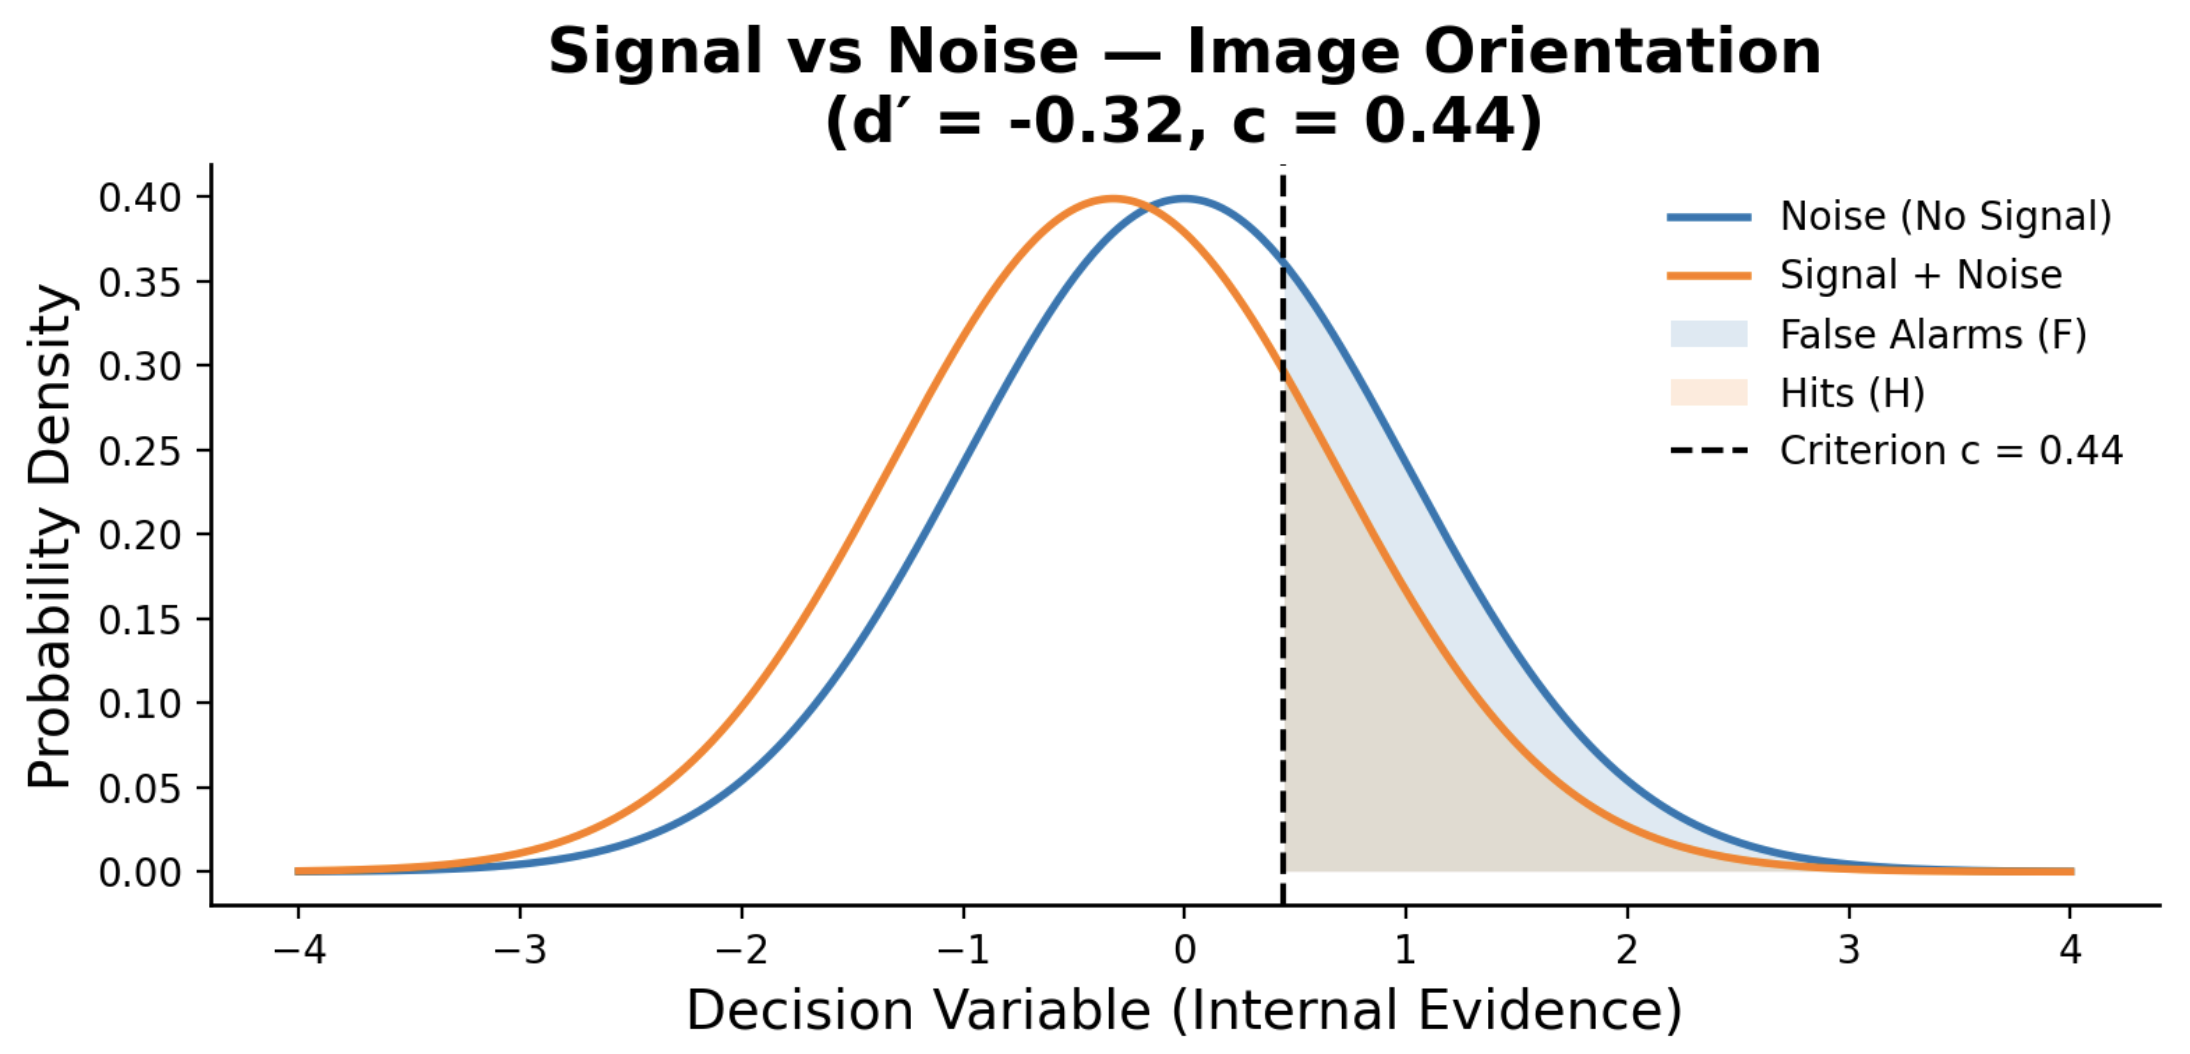
\includegraphics[width=0.75\textwidth]{figures/ImageOrg.png}
    \caption{Signal and noise distributions in the Image Orientation (Yes/No) task.}
    \label{fig:image_orientation_sdt}
\end{figure}

The Gaussian distributions represent my subject's internal evidence for
``upright'' (signal-present) versus ``inverted'' (signal-absent) image trials. 
The overlap between the distributions is substantial ($d'=-0.32$), indicating low 
discriminability between the two categories. The criterion ($c=0.44$) lies to the 
right of the midpoint, showing a slightly \textit{conservative bias} — the participant 
tended to respond “upright’’ only when confident. Shaded regions indicate false 
alarms (blue) and hits (orange), which correspond to the decision areas in the 
equal-variance signal detection model.

\begin{figure}[H]
    \centering
    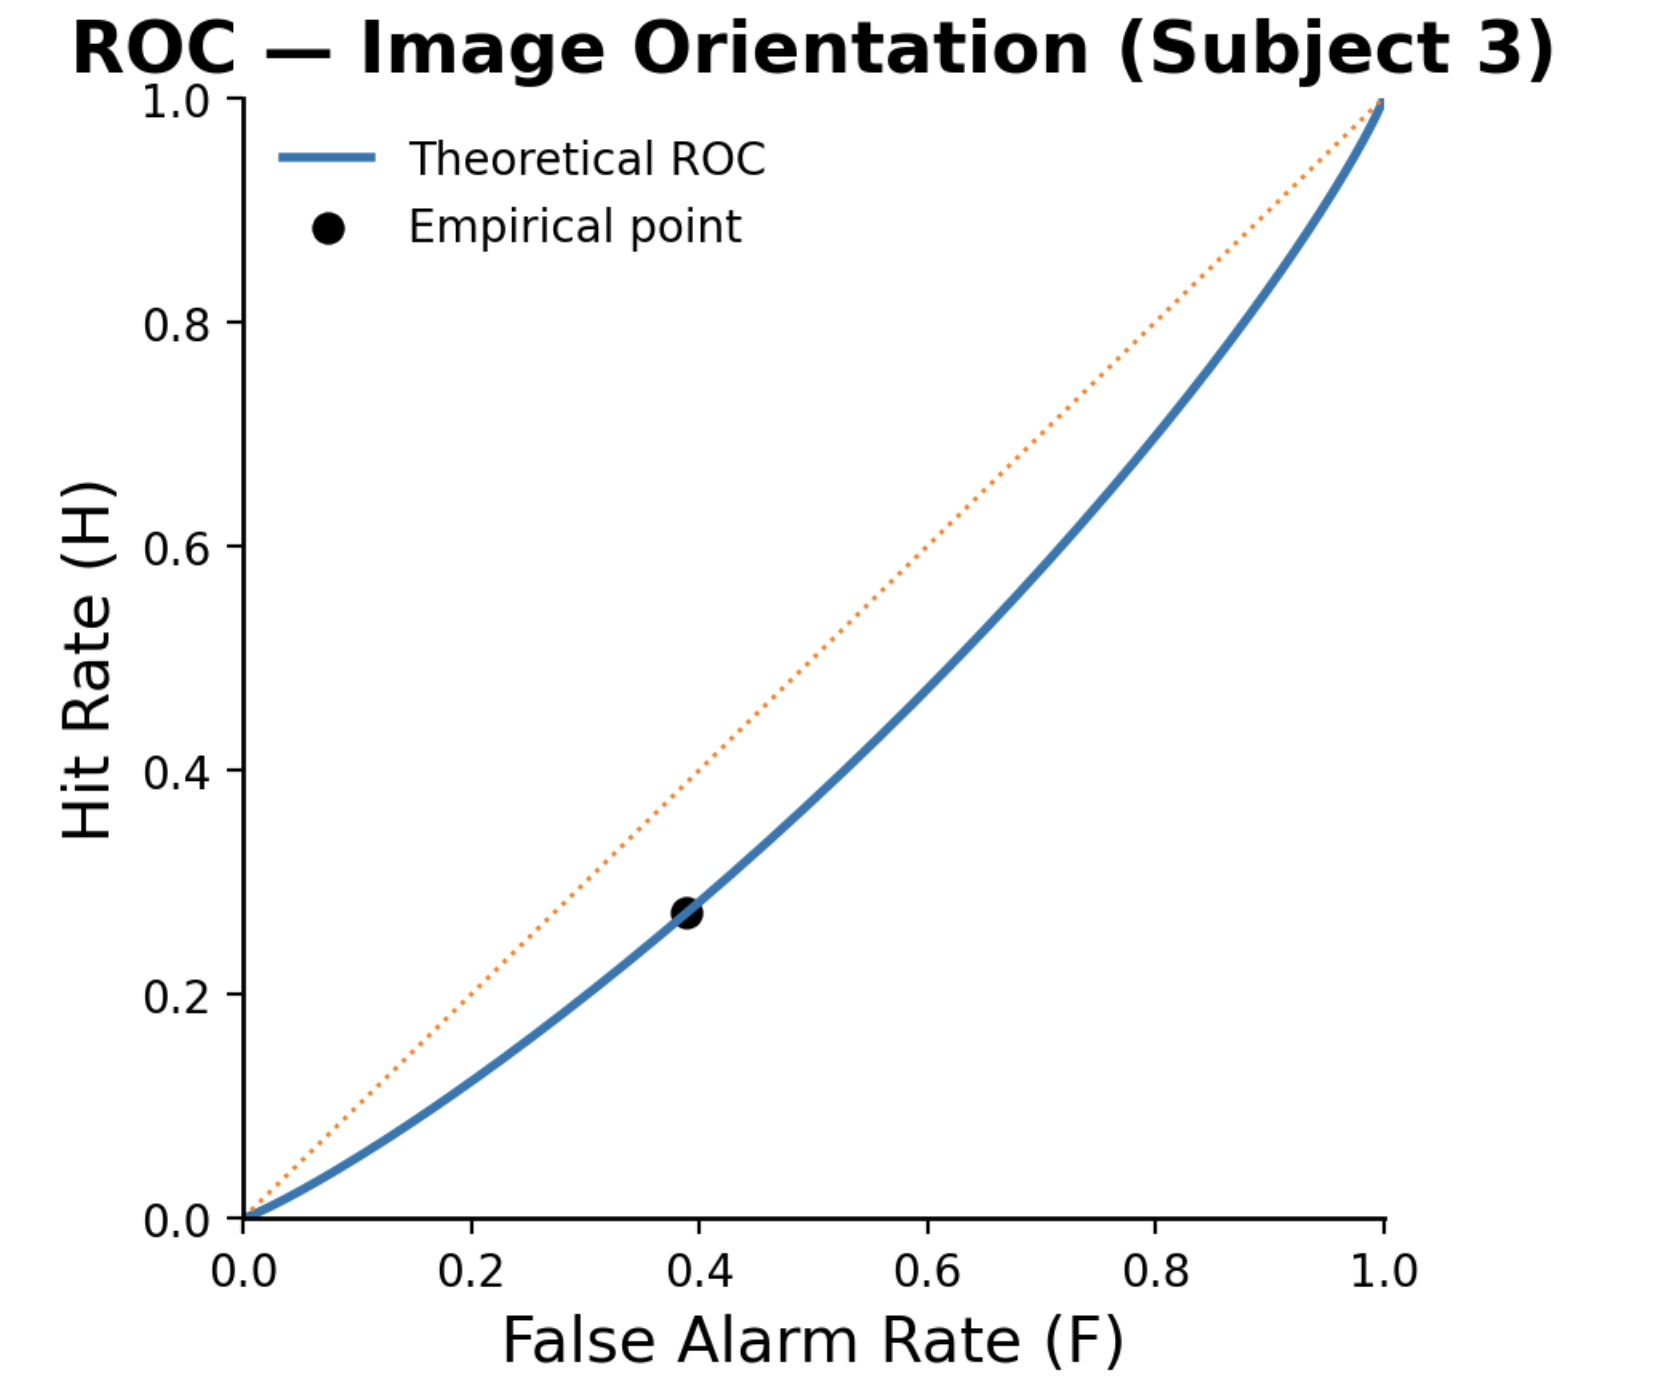
\includegraphics[width=0.55\textwidth]{figures/ImageOrgROC.png}
    \caption{Receiver Operating Characteristic (ROC) curve for the Image Orientation task.}
    \label{fig:image_orientation_roc}
\end{figure}

The ROC curve shows the relationship between hit rate ($H=0.27$) and false-alarm rate ($F=0.39$). 
The empirical operating point (black dot) lies close to the chance diagonal, 
consistent with random performance. The equal-variance SDT model (blue line) 
accurately captures the observed pattern, confirming that the participant's 
responses were statistically indistinguishable from chance. 
Overall, $d'=-0.32$, $c=0.44$, and accuracy $=0.43$ (95\% CI [0.29--0.57], $p=0.43$) 
provide no evidence for ESP or clairvoyant ability.

    
\end{itemize}